\chapter{Approche modulaire des réseaux de neurones}
\graphicspath{{01-Modularite/}}

%%%%%%%%
% Intro du chapitre : Trouver un questionnement, un exemple qui parle de modularité dans les systèmes biologiques:  
%
%%%%%%%%%%%%%%%%%%%%%
L'idée de ce chapitre est d'inscrire nos travaux dans le coté modulaire des réseaux de neurones. Il nous foudra donc définir proprement ce qu'on appelle modularité, et définir les motivations pour créer une architecture modulaire. 
D'une part, de nombreux modèles biologiques présentent des architectures modulaires. Notre conception du monde se présente en fait sous une forme de modularité.

En tant qu'humain, nous comprenons le monde de notre point de vue, en le décomposant pour qu'il semble accessible : en effet notre raisonnement est modulaire, notre système social, groupes d'individus, etc, comme l'explique par exemple \cite{Morowitz1995TheMT} dans "How a mind resides in the brain".
Nos contructions sont modulaires : programme informatique ... Il est difficile de concevoir et surtout de comprendre, en tant qu'humain, un système qui ne serait pas décomposable en modules. Prenons comme exemple les réseaux de neurones profonds : la compréhension  et l'interprétabilité ces programmes est un défi de la recherche actuelle. Pour cette interprétation, on cherche des éléments symboliques, des groupes, des communautés. 
La décomposition des sciences elles même, par exemple, nous permet de trouver des solutions aux problèmes a des échelles différentes. Le programmeur n'a pas besoin de comprendre en profondeur quels transistors composent les circuits; l'expert.e en electronique n'a pas besoin de d'abord résoudre les équations qui régissent les mouvements ioniques au sein des transistors pour concevoir des circuits, etc. Seuls les principes régissant les comportement globaux d'un système commme le transistors ont besoins d'être connus pour utiliser ces sytèmes dans une tâche; tâche qui consituera également un module dans son ensemble et qui sera régie par des principes généraux, du transitor à l'utilisation d'un logiciel de dessin graphique. 
Mais est ce que cette hiéarchie modulaire est essentiellement subjective ? A priori non. Une organisation modulaire est présente et calculable dans de nombreux systèmes.


Présentation d'exemples de théories dérivées d'une modularité bio-inspirée. 
Brooks \cite{brooks_sumsumption_85}

Les modules sont également associés aux systèmes complexes. De nombreux travaux sont ainsi réalisés à la frontière entre domaines, 
Réseaux associés aux systèmes complexes, interactions


%%%%%%%%%%%%%%%%%%%%%%%%%%%%%%%%%%%%%%%%%%%%%%%%%%%%%%%%%%%%%%%%%%%%%%%%%%%
% SECTION 1 introduction via la biologie, exemples 
%%%%%%%%%%%%%%%%%%%%%%%%%%%%%%%%%%%%%%%%%%%%%%%%%%%%%%%%%%%%%%%%%%%%%%%%%%%%


\section{La modularité, répandue dans les système biologiques}

\subsection{Systèmes complexes }

Les systèmes, dans leur échelles, sont donc complexes. Si on peut décomposer des systèmes pour les étudier, ils restent liés au sein d'un vaste écosystème. Ainsi, l'étude de la modularité des systèmes est présente au sein des approches biologiques.

"Un système complexe est un ensemble constitué d'un grand nombre d'entités en interaction dont l'intégration permet d'achever une mission commune. Les systèmes complexes sont caractérisés par des propriétés émergentes qui n'existent qu'au niveau du système et ne peuvent pas être observées au niveau de ces constituants. (wikipedia)". Ces constituants interagissent par des règles locales qui sont souvent simples, mais dont l'interaction forme des propriétés émergentes. Complexe ne veut pas dire que les relations et interactions sont difficiles a exprimer : un système est complexe du point de vue d'un observateur, mais les règles locales sont souvent simples. 
-> Exemple fourmilière, 
L'Emergence de patterns et de phénomènes d'auto-organisation (turing patterns) \cite{turing52} qui sont même utilisés pour qualifier le système complexe. 

Il n'y a a priori pas de définition commune concernant ce qu'on appelle un système complexe et comment le mesurer. On pourrait plutot voir la complexité comme une façon d'étudier un objet. 

Exemple de définition : complexité de Kolmogorov qui évalue la complexité par la taille du plus petit module permettant d'engendrer l'objet; une façon de définir la complexité parmi d'autres. Autre exemples : ??



Systèmes liés par des équations d'évolution et des conditions initiales. 

Qui dit système complexe dit système modulaire ?

Réseaux sociaux, communautés de fourmis, autant d'exemples montrant une emergence auto-organisée de modules. 

\subsection{Le cerveau, réseau modulaire fondamental}

L'étude des réseaux biologiques, notamment, a fait émerger l'idée d'architectures modulaires. Si on considère en plus la notion d'apprentissage dans les réseaux modulaires, l'étude des cerveaux est une mine d'information et de questionnement quant aux structures et propriétés le permettant. 
Les premières propositions d'études du cerveau humain datent du début du XXeme siècle. Déjà, un découpage en aires est proposé pour expliquer le fonctionnement de cet organe, notamment avec les travaux de Broca et Wernicke qui mettent en lumière des zones du cerveau qui semblent responsable du langage. Le modèle connexioniste du cerveau, formalisé à partir de ces travaux par Geschwind dans les années 60 , décompose ainsi le langage en plusieurs fonctions : la compréhension, la lecture et l'action de parler. Ce modèle n'est plus vraiment utilisé, mais l'idée de décomposition en modules reste valable.
Avec l'avènement des outils d'imagerie, le cerveau a pu être cartographié plus préciséement en un ensemble d'aires, agissant comme modules fonctionnels au sein d'une structure complexe; ces aires sont elles mêmes composées de modules distincts.
L'étude des aires et des connexions entre zones du cerveau, comme~\cite{primate_cortex_91} dans le cas du cortex visuel du primate, découpent les zones activée pour la vision en modules distincts, et montrent que ces modules sont connectés. Ces connexions, en fonction des modules, sont réciproques ou non. Les "pathsways" du cerveau désignent des modules fortement connectés. Leur détection expérimentale est réalisée en relevant des indicateurs de dépendance (corrélation, ..., en fonction des méthodes utilisées). Ainsi, \cite{Rolls2002ComputationalNO} précise la structure des différentes aires cérébrales en présentant les connexions au sein de ces aires, par exemple la structure présentée en figure~\ref{fig:cortex2} pour l'aire visuelle. 
Les connexions du cerveau sont présentes à différentes échelles: des pathsways existent ainsi au sein de l'aire visuelle du cerveau, mais des boucles de rétroaction entre zones cérébrales sont présentes à plus grande échelle, par exemple la boucle baso-thalamo_corticale. 

Le cerveau est ainsi présenté en modèle et motivation principale lorsqu'il s'agit de construire des réseaux de neurones artificiels. 
- Nombreuses études s'appuient sur le système modulaire : le cerveau \cite{primate_cortex_91,mountcastle_columnar_1997,binzegger05}

- Modularité structurelle : exemple du cortex visuel

- Connexions : hiérarchiques ou non, et feedback, ex boucle baso thalamo corticale, ou au sein des aires comme le cortex visuel.

- Modularité hiérarchique( modules de modules) -> Ajouter infos depuis l'article qui parle de modules hiérrchiques. 

%\begin{figure}
%\centering
%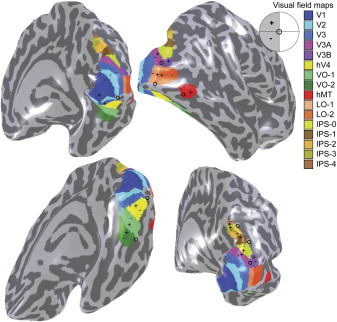
\includegraphics[width=0.5\textwidth]{visual_field_maps.jpg}
%\caption{Représentation de 16 aires cérébrales liées au cortex visuel dans le cerveau humain, voir \cite{WANDELL2007366}}
%\label{fig:cortex}
%\end{figure}

\begin{figure}
\begin{minipage}{0.5\textwidth}
\centering
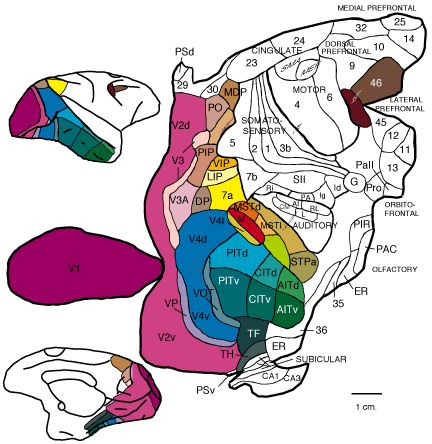
\includegraphics[width=0.6\textwidth]{FVE_fig2map.png}
\caption{carte aplanie des aires du cortex visuel du macaque \cite{primate_cortex_91}}
\label{fig:cortex1}
\end{minipage}
\begin{minipage}{0.5\textwidth}
\centering
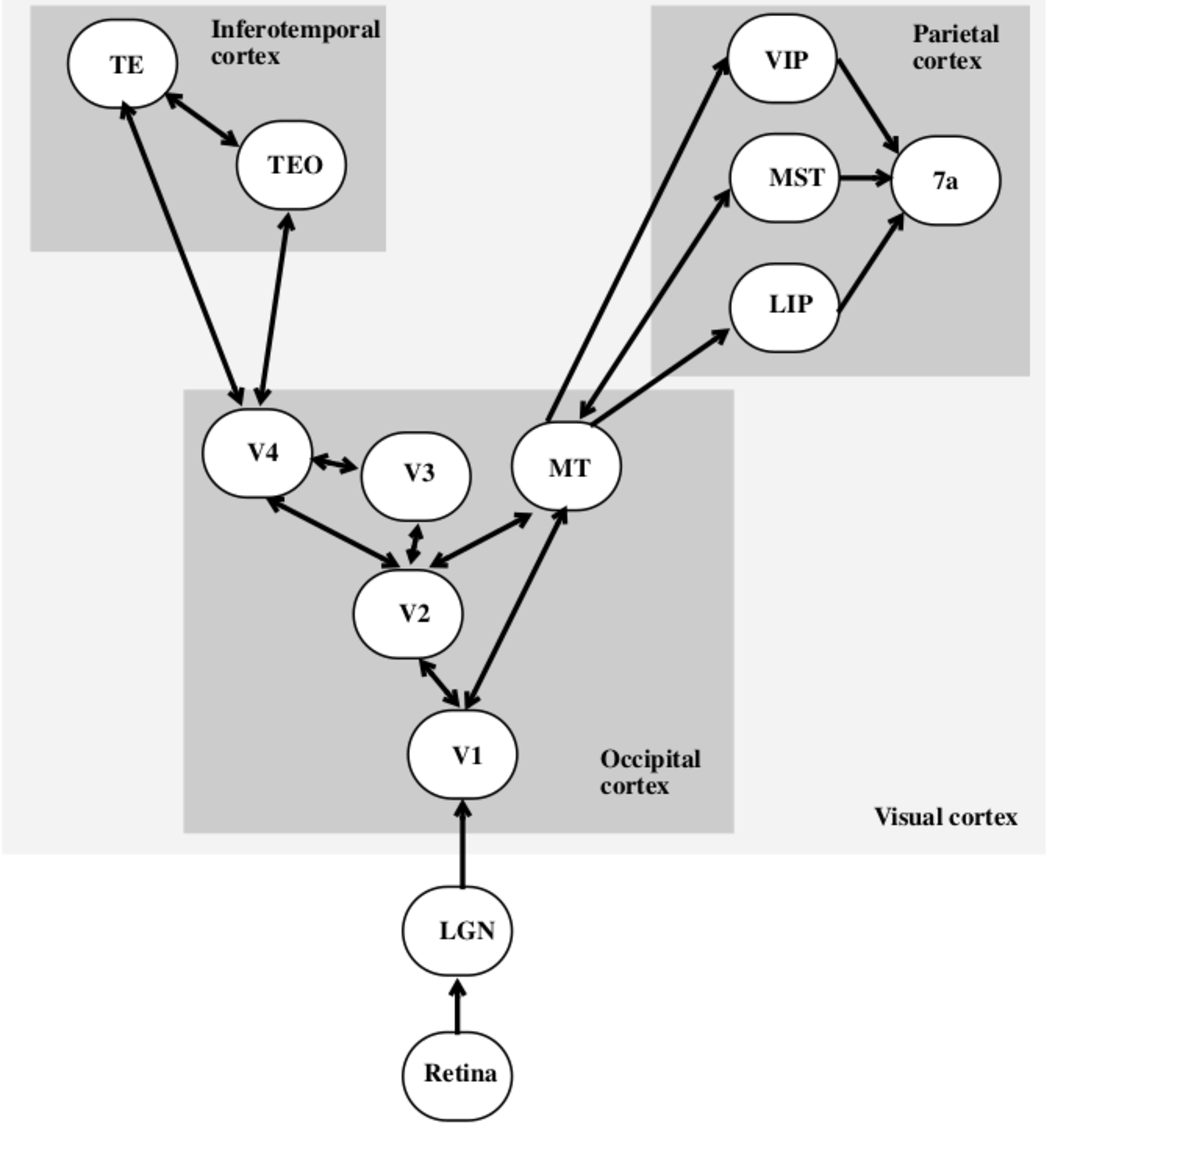
\includegraphics[width=0.6\textwidth]{rolls_pathways.pdf}
\caption{pathways dans le cortex visuel du macaque, entre les aires listées figures de gauche. \cite{Rolls2002ComputationalNO}}
\label{fig:cortex2}
\end{minipage}
\end{figure}


%Ajouter figure du cerveau avec le schéma des aires

TODO : que signifient pathways streams (vite fait )
Finalement : 
Cerveau présente ce qu'on peut appeler des modules, avec des connexions entre eux, avec rétroaction. 

Leur mesure peut etre structurelle (regarder les structures de neurones), ou fonctionnelle : quelles aires s'activent pour une fonction ? \\
Détail des types de modularité en parties suivantes. 

\subsection{Des réseaux et des modules dans tous les systèmes biologiques}

%%%%%%%%%%%%%%%%%%%%%%%%%%%%%%%%%%%%%%%%%%%%%%%%%%%%%%%%%%%%%%%%%%%%%%%%%%%%%
% SECTION 2 : définitions et propriétés
%- Tour d'horizons des définitions : en bio, en ingénieurie. Auto-organisation, conséquence de la modularité ? 
%- Taxonomie : fonctionnelle, stucture modulaire,emergence 
%- Position de l'autrice du manuscrit sur la modularité, intéret des différentes modularités
%- Discussion : est ce que notre esprit modulaire veut trouver de la modularité a tout prix ? ( quand la mod est fonctionnelle, peut etre biais de nos représentations ? Mais, on observe assez objectivement des modules physiques via les connexions dans de nombreux réseaux. Evolution l'a fait comme ca, probablement une réponse globale a un problème. 
%- Echelles de la modularité. 
%- Activation d'autres modules
%- Mutli-modalité - un mot, rappel dans une autre partie
%%%%%%%%%%%%%%%%%%%%%%%%%%%%%%%%%%%%%%%%%%%%%%%%%%%%%%%%%%%%%%%%%%%%%%%%%%%%%%%

\section{Quelle définition de la modularité ?}

Il s'agit de tirer une définition claire de ce qu'on appelle modularité. Entre l'étude des systèmes biologiques et l'ingénieurie des réseaux de neurones, l'aspect modulaire des réseaux et plus généralement des systèmes peut se définir de plusieurs manières. 

\subsection{Modularité structurelle}

Lorsque le système possède une structure définie de réseau, typiquement un réseau de neurones, on peut définir une modularité en terme de graphe. La définition de cette modularité dépend un peu des réseaux que l'on cherche a étudier; on va essayer de lister ici les différents aspects qui se cachent sous le terme de "graphe modulaires", et dans quels domaines ils sont utilisés.

\subsubsection{Mesurer la modularité structurelle d'un réseau}
clustering coefficient
proximity ratio
scale free networks

\cite{Harriger2012RichCO}-> mesure modularité dans le cerveau, partie "méthodes" explique les méthodes de mesure de modularité. TODO les lister

Modularité : détection de communautés.


\subsubsection{Réseaux en "petit-monde" et réseaux sans échelle}
Definition: type de graphe dans lequel la distance moyenne entre deux noeuds est proportionnelle à log(N), N le nombre de noeuds. C'est à dire, un graphe dans lequel on trouvera un chemin assez court entre n'importe quels noeuds. 
Particularités : forme souvent des cliques ( sous graphes fortement connexes), donc une structure modulaire. Par contre, tous les réseaux small world ne sont pas necessairement modulaire. 
Souvent admis que le cerveau en tant que réseau de neurones est small world. 

\begin{figure}
\begin{minipage}{0.5\textwidth}
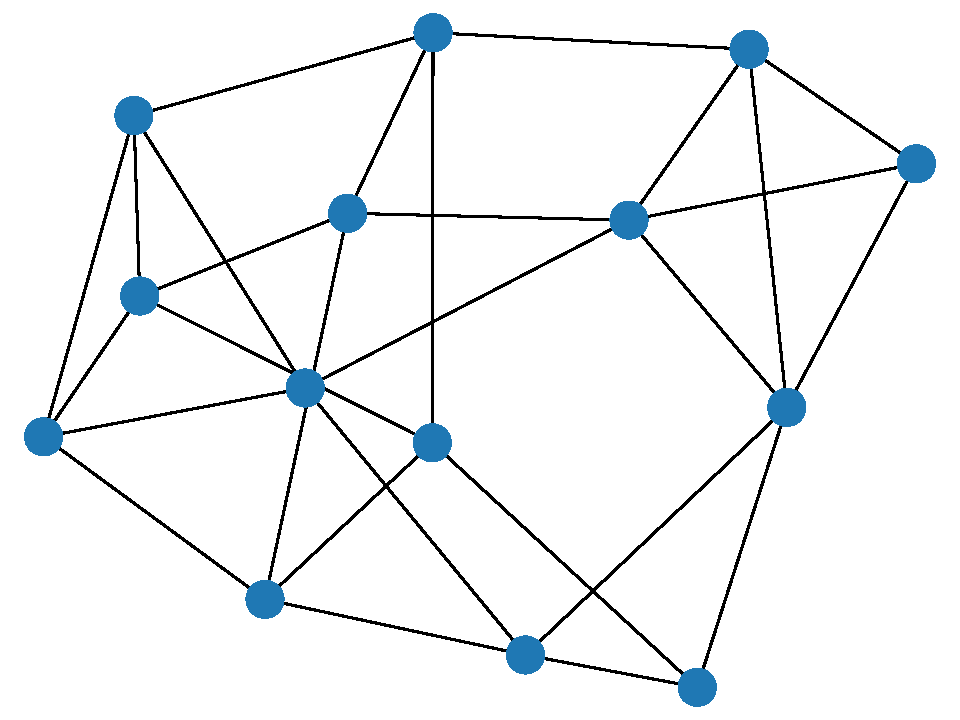
\includegraphics[width=\textwidth]{watts_strogatz.pdf}
\caption{Réseau aléatoire "petit-monde" créé avec l'algorithme de Watts-Strogatz}
\end{minipage}
\begin{minipage}{0.5\textwidth}
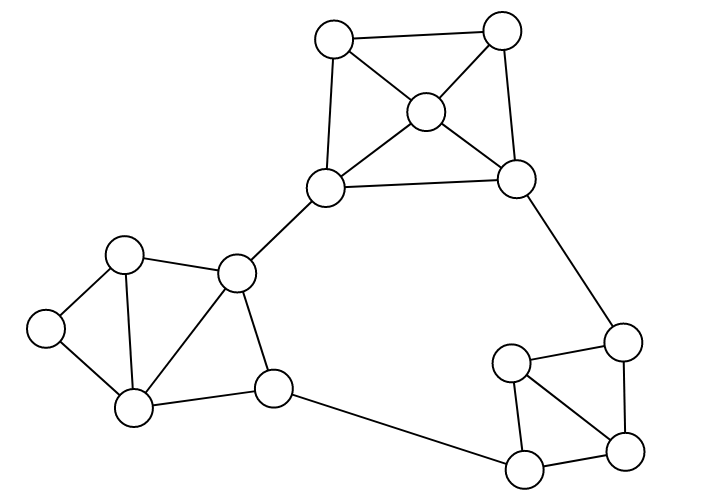
\includegraphics[width=\textwidth]{small_world_net.png}
\caption{Réseau modulaire : il possède une propriété de "petit monde" mais des modules, zones fortement connectées, sont identifiables.}
\end{minipage}

\end{figure}
\subsubsection{Modularité auto-similaire}

Exemples ?? \cite{Meunier2010ModularAH}
Modularité hiérarchique présente l'avantage de maintenir une activité dans le réseau sans que ca ne colonise tout ni ne s'eteigne, ce qui est nécessaire pour la computation. 




\subsubsection{Def}
\cite{Hilgetag2015IsTB} : différencie réseaux small world et réseaux hiararchique modulaires, et statue qu'un réseau peut etre "hiérarchique modulaire" même s'il n'est pas small world, mais possède une dimension topologique finie. 
\cite{Meunier2010ModularAH} : statue que un réseau modulaire est small world,


En bref : 
- techniques de detection de communautés sur des graphes pour detecter une modularité.
- Certaines structures se distinguent parmi les graphes modulaires :  small-world, scale-free, hiérarchique. ces structures se recoupent.^
- Au niveau du cerveau, on n'est pas hyper d'accord sur le type de modules, mais les expés montrent une structure. 

\subsection{Modularité fonctionnelle}


\subsection{Modularité temporelle}

La modularité s'associe aux séquences dans le cerveau. On peut donc raisonnablement définir 

\subsection{Emergence d'une modularité et auto-organisation}

Est ce que l'auto-organisation d'un système dénote d'une modularité ? 

%%%%%%%%%%%%%%%%%%%%%%%%%%%%%%%%%%%%%%%%%%%%%%%%%%%%%%%%%%%%%%%%%%%%%%%%%%%%%%%%%%%%%%%%%%%%%%%%%%%%%%%%%%%%%%%%%%%%%%%%%%%%%%%%%%%%%%%%
% SECTION 3: quel intéret à utiliser des architectures modulaires pour l'apprentissage ? 
% - 
%%%%%%%%%%%%%%%%%%%%%%%%%%%%%%%%%%%%%%%%%%%%%%%%%%%%%%%%%%%%%%%%%%%%%%%%%%%%%%%%%%%%%%%%%%%%%%%%%%%%%%%%%%%%%%%%%%%

\section{Intérêt computationnel des réseaux modulaires}

Barabasi : Hypothèse que les réseaux small world présentent un avantage evolutionnaire.

\subsubsection{réponse a un problème de contrainte physiques, énergétiques}

- Parallelisme, calcul et small world networks : réponse a un problème de contrainte physiques, énergétiques. 
- Calcul distribué 
- Automates cellulaires  ?


\subsection{Types de connexions}

Opaque vs tout savoir

\subsection{Modularité et émergence d'un apprentissage ? }

La modularité est liée a la complexité des systèmes, donc l'emergence de comportements chaotiques et/ou synchronisés. 
SYSTEMATIC GENERALIZATION : WHAT IS REQUIRED
AND CAN IT BE LEARNED ? : 
Our findings show that the generalization of modular models is much more systematic and that it is highly sensitive to the module layout, i.e. to how exactly the modules are connected.

Simplicité de la modularité : exemple de construction des fractales, exemple du rigaudon

%%%%%%%%%%%%%%%%%%%%%%%%%%%%%%%%%%%%%%%%%%%%%%%%%%%%%%%%%%%%%%%%%%%%%%%%%%%
% SECTION 4 En pratique, ou en est on des réseaux de neurones modulaires ?
%%%%%%%%%%%%%%%%%%%%%%%%%%%%%%%%%%%%%%%%%%%%%%%%%%%%%%%%%%%%%%%%%%%%%%%%%%%%%ùù

\section{Réseaux de neurones modulaires}

- Challenges et intérêt potentiel des réseaux de neurones modulaires ? -> Evolution (wertmer, meunier) : pousser plus loin pour etre au jus sur les challenges actuels ( voir du coté du deep : quelles sont les motivations et les challenges ? 



\subsection{Deep Learning}

Boites noires qui ont des performances remarquables sur tous les domaines, leur représentation et compréhension est quant à elle toujours un challenge.

\subsubsection{Il existe des réseaux modulaires}
- Réseaux qui apprennent a s'organiser en modules. Interet. Limites ? Performances ? \cite{Andreas2016NeuralMN,Kirsch2018ModularNL}
"The NMN approach is intuitively appealing but its
widespread adoption has been hindered by the large amount of domain knowledge that is required
to decide (Andreas et al., 2016) or predict (Johnson et al., 2017; Hu et al., 2017) how the modules
should be created (parametrization) and how they should be connected (layout) based on a natural
language utterance. Besides, their performance has often been matched by more traditional neural
models" ( systematic generalization article ) 

\subsubsection{Utiliser des modules pour mieux représenter les réseaux de neurones profond}
- Trouver des modules dans les réseaux pour les expliquer ? \cite{Watanabe2018ModularRO,Csordas2021AreNN}
are neural net modular : "it uses different modules for very different functions = Pspecialize," et "it uses the same module for identical functions that
may have to be performed multiple times = Preuse"
- Reconciling deep learning with symbolic artificial intelligence: representing objects and relations(2019)
Pb du deep learning = Data inefficiency (comparé a l'humain);Poor generalisation; Lack of interpretability.

\subsection{Réseaux auto-organisés}

Les réseaux auto-organisés sont directement inspirés des réseaux biologiques. Au sein de ces réseaux
Plus qu'en deep learning, les réseaux de neurones auto-organisés
- Auto-organisation prend une profonde inspiration biologique, tout comme les modules.
- Exemple de réseaux auto-organisés modulaires : développer dans la partie suivante.
\begin{figure}
\centering
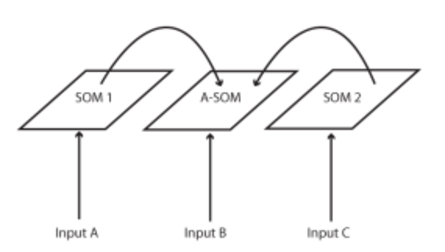
\includegraphics[width=0.5\textwidth]{asom}
\caption{A-SOM model \cite{johnsson_associative_2009}}
\end{figure}
\begin{figure}
\centering
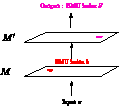
\includegraphics[width=0.5\textwidth]{hsom}
\caption{HSOM model \cite{LampinenClusteringPO}}
\end{figure}


\cite{LampinenClusteringPO}
\cite{parisiLL}

\subsection{Construire une architecture modulaire}

A mettre dedans : 

- Réseaux top down / modulaires ? définition, a quel point un réseau est modulaire, qu'est ce qu'on appelle réseau modulaire ? 
Fonction définies au préalable vs émergence des fonctions. 
Modules définis au préalable vs émergence des modules. 


%%%%%%%%%%%%%%%%%%%%%%%%%%%%%%%%%%%%%%%%%%%%%%%%%%%%%%%%%%%%%%%%%%%%%%%%%%%%%%%%
% SECTION 5 : proposer des enjeux par rapports au réseaux listés précedemment 
%%%%%%%%%%%%%%%%%%%%%%%%%%%%%%%%%%%%%%%%%%%%%%%%%%%%%%%%%%%%%%%%%%%%%%%%%%%%%%%%


\section{Enjeux d'une architecture modulaire de SOMs}

On connait plutot bien les SOM, mais on sait que des comportements nouveaux peuvent émerger lorsqu'on met en interaction des systèmes étudiés séparément. 
On peut donc se poser la question des comportements qui peuvent survenir dans ce cas.

Dans les structures de cartes étudiés, modularité forte dans le sens ou les fonctions des modules sont prédéfinies. Si on ne fournit que les règles d"interaction, ou est ce qu'on se situe ? 
 
 
Position du manuscrit : architecture 
%%%%%%%%%%%%%%%%%%%%%%%%%%%%%%%%%%%%%%%%

Plan de la partie ! 

 

\begin{enumerate}
\item Intro : Notre monde est modulaire, en tout cas nous l'interprétons en tant que tel. Proposé déjà dans les années 60 - breve histoire des réseaux de neurones ?
Remarquer que nous, observeur, raisonne et se construit modualairement. Il nous est difficile de concevoir les choses autrement. 
Les disciplines sientifiques par ex, un domaine obéit a des principes
\item Qu'appelle t-on la modularité ? Définitions claires et propriétés
	\begin{itemize}

		\item Definition
			\begin{enumerate}
			\item Structurelle, dans les systèmes réseaux
			\item Fonctionnelle, dans les systèmes dont on ne connait pas la structure ?\\
			\item Temporelle / mais est ce que le temps ce n'est qu'une dim de plus
			\item Modularité hiérarchique attention : deux defs a hiérarchiques. Soit c'est une histoire de connexions, soit d'auto-similarité. On parle nous de l'auto similarité !!! Au contraire l'autre forme de hiérarchie n'est pas observée en bio.
			\end{enumerate}
		
		\item Propriétés de la modularité 
			\begin{enumerate}
			\item Auto-organisation
			\item Types de connexions
			\item Emergence
			\end{enumerate}
	\end{itemize}	
\item Exemples Biologiques et computationnels
	\begin{enumerate}
	\item Biologie : opti evolution a priori...
	\item Computationnel : pareil.
	\end{enumerate}
	
\item Maintenant qu'on sait ce que sont les systèmes modulaires, en quoi on peut faire de l'apprentissage avec ? Quels sont les intérêts ?
	\begin{enumerate}
		\item Exemples de réseaux auto-organisés
		\item Exemples de réseaux de neurones : deep learning
	\end{enumerate}

\end{enumerate}





